\documentclass[tikz, border=5pt]{standalone}
\usetikzlibrary{arrows.meta, shapes, positioning, decorations.pathmorphing, patterns}

\tikzset{
  spring/.style = {
    decoration = {aspect=0.3, segment length=2mm, amplitude=2.5mm, coil, pre length=4mm, post length=3mm},
    decorate
  }
}

\begin{document}

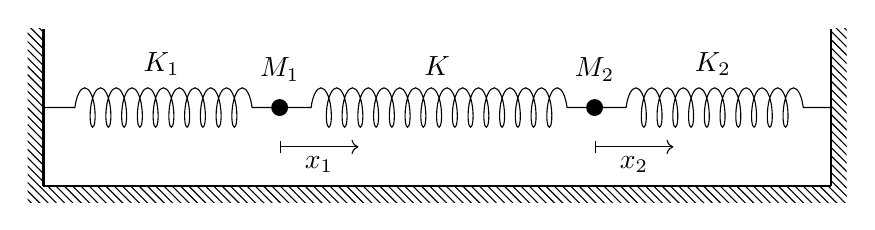
\begin{tikzpicture}

  %% Hamiltonian formulation

  % Walls
  \draw[thick] (-5,0) -- (5,0);
  \draw[thick] (-5,0) -- (-5,2);
  \draw[thick] (5,0) -- (5,2);
  \fill[pattern = north west lines] (-5,0) rectangle (-5.2,2);
  \fill[pattern = north west lines] (5,0) rectangle (5.2,2);
  \fill[pattern = north west lines] (-5.2,-0.2) rectangle (5.2,0);

  % Masses
  \draw[fill=black] (-2,1) circle (0.1) node[above, yshift=6] {\(M_1\)};
  \draw[fill=black] (2,1) circle (0.1) node[above, yshift=6] {\(M_2\)};

  % Springs
  \draw[spring] (-5,1) -- (-2,1) node[midway, above, yshift=8] {\(K_1\)};
  \draw[spring] (-2,1) -- (2,1) node[midway, above, yshift=8] {\(K\)};
  \draw[spring] (2,1) -- (5,1) node[midway, above, yshift=8] {\(K_2\)};

  % Displacements
  \draw[|->] (-2,0.5) -- node[below] {\(x_1\)} (-1,0.5);
  \draw[|->] (2,0.5) -- node[below] {\(x_2\)} (3,0.5);

\end{tikzpicture}

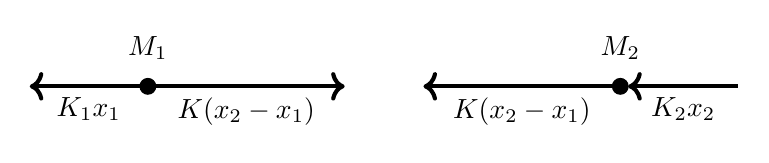
\begin{tikzpicture}

  %% Newtonian formulation

  % FBD of M_1
  \draw[fill=black] (0,0) circle (0.1) node[above, yshift=6] {\(M_1\)};
  \draw[->, line width=1.5pt] (0,0) -- (-1.5,0) node[midway, below] {\(K_1 x_1\)};
  \draw[->, line width=1.5pt] (0,0) -- (2.5,0) node[midway, below] {\(K(x_2-x_1)\)};

  % FBD of M_2
  \begin{scope}[xshift=6cm]
    \draw[fill=black] (0,0) circle (0.1) node[above, yshift=6] {\(M_2\)};
    \draw[<-, line width=1.5pt] (0+0.1,0) -- (1.5,0) node[midway, below] {\(K_2 x_2\)};
    \draw[->, line width=1.5pt] (0,0) -- (-2.5,0) node[midway, below] {\(K(x_2-x_1)\)};
  \end{scope}

\end{tikzpicture}

\end{document}
